\documentclass[conference]{IEEEtran}
\IEEEoverridecommandlockouts
\usepackage{cite}
\usepackage{amsmath,amssymb,amsfonts}
\usepackage{algorithmic}
\usepackage{graphicx}
\usepackage{textcomp}
\usepackage{xcolor}
\def\BibTeX{{\rm B\kern-.05em{\sc i\kern-.025em b}\kern-.08em
    T\kern-.1667em\lower.7ex\hbox{E}\kern-.125emX}}
\begin{document}

\title{Genetic Algorithm for a Self-Driving Car*\\
{\footnotesize \textsuperscript{*}Note: For this particular case, the algorithm evolved in a 2D complex environment.}
}

\author{\IEEEauthorblockN{Fabio Oliveira}
    \IEEEauthorblockA{\textit{Msc. Applied Artificial Intelligence} \\
        \textit{Polytechnic Institute of Cavado and Ave}\\
        Barcelos, Portugal \\
        fabiodiogo29@gmail.com}
}

\maketitle

\begin{abstract}
    The challenge with self-driving cars is to create a model that converts sensors data (such as cameras or proximity sensors) into actions.
    This way the car can react to its changing environment and make the right decisions. Games offer a suitable testbed where new methodologies
    and algorithms can be tested in a near-real life environment. For example, in a car driving game, using transfer learning or other techniques
    results can be generalized to autonomous driving environments. In this paper, we propose a agent based on a genetic algorithm that learns to
    drive autonomously in a complex environment given real time data from the car sensors. In the literature \cite{neelarghya_2021,mandav_2018,patel_2021}, Neural Networks is the most
    promising technique used to parse these sensors data. For this particular case we'll use a 2nd order polynomial function to convert the data
    from three sensors into one action (degree of turn). To simulate the car and the environment we've put together a car game simulator with Pygame.
    The code is available at \textbf{\textit{github.com/fabioo29}}.
\end{abstract}

\begin{IEEEkeywords}
    Artificial Intelligence, Neural Networks, Genetic Algorithm, Pygame
\end{IEEEkeywords}

\begin{figure}[b]
    \centerline{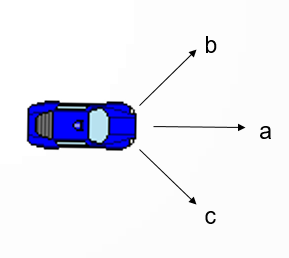
\includegraphics[width=40mm,scale=2]{assets/car-sensors.png}}
    \caption{Population car sensors(whiskers)}
    \label{fig:car-sensors}
\end{figure}

\section{Introduction}
Today, as the world is ushering into the era of automating things, one of key product of the industries which is yet
to be automated completely is a vehicle which is also intelligent. According to Pcmag \cite{pcmag_unknown}, "An autonomous vehicle is a
computer-controlled car that drives itself". There are many industries which are leading the research in autonomous
vehicles, some of the most prominent are Google, Tesla and NIO. Research nowadays is inclining towards becoming leader
in the new age of driver-less car. However, the current driver-less car is yet far from being the intelligent autonomous
car. Some autonomous vehicles uses LiDAR (Light Detection And Ranging) technology, that measures distance to a
target by illuminating the target with pulsed laser light and measuring the reflected pulses with a sensor. Otherwise, tesla mainly focus is
too use video for the environment perception. For this work, as mentioned before, each population car will have three sensors acting as distance
sensors and the goal of the car is to drive through all the track without crashing into the wall.
The motivation for this work came from applied artificial intelligence Msc. degree teacher in Fundamentals of Artificial Intelligence,
Alberto Simões, who proposed the idea of using a genetic algorithm to create a self-driving car with a 2nd order polynomial function
acting as a controller for the car instead of using neural networks to control it like a typical state-of-the-art autonomous car.
The following paper is organised as follows, Section 2 covers the topics and methodologies used for this approach, Section 3 explains about the proposed
method and algorithms used to develop the autonomous driving agent, Section 4 covers the experiments and results obtained from the
state of the art method used, Section 5 concludes the paper by iterating over the findings in the project.

\section{Metodologies}
\subsection{Genetic Algorithm}
Genetic Algorithm is a search metaheuristic that is inspired by Charles Darwin’s theory of natural evolution.
This algorithm reflects the process of natural selection where the fittest individuals are selected for reproduction
in order to produce offspring of the next generation. A genetic algorithm process consists in a series of steps as follows.

\subsubsection{Generate Initial population}
For the algorithm to evolve it is necessary to generate an initial population. The initial population is a set of individuals,
where each individual is controlled by an Agent and each Agent is characterized by a set of Genes represented as a value between
-1 and 1. A set of genes is known as a Chromosome. The population with which we start is called the Initial Population.

\subsubsection{Evaluation}
A Fitness function is a system that determines how fit (the ability of an individual to compete with other individuals)
an individual is. It gives a fitness score to each individual which helps quantify the performance.
This function is executed over the performance of the population to quantify and compare the individuals performance.
The fitness used for this particular case is the distance traveled by the car. So, it means that those cars who traveled
the most will rank higher on the selection process.

\subsubsection{Selection}
The process of picking the “fittest” (based on the fitness score generated during Evaluation phase) individuals for
producing the next generation (i.e. the new population for the next cycle of evaluation and reproduction). There isn’t
a strict cut-off based on the fitness score, but state-of-art mehtods typically mention selection based on probabilities
(higher the fitness score, higher the probability to get selected), tournament selection and roulette wheel selection.
After a few investigation of the literature and tests on the subject, we’ve decided delete between 60 and 85% of the population
which ended up working well in our case.

\subsubsection{Crossover}
The process of mixing the genes of the pair of individuals chosen to produce a new pair of individual is called
Crossover or Genetic operation. This process is continued to create a new population. Crossover can be performed in
different methods such as one-point crossover, two-point crossover, uniform crossover and so on.
We ended up using uniform crossover between top two ranked cars (by fitness) to produce a new pair of cars (each new car gene
has 0.50 probability to be selected from the top one car or from the top two car) as illustrated in the figure \ref{fig:crossover}.

\begin{figure}[t]
    \centerline{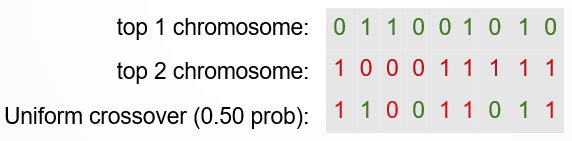
\includegraphics[width=80mm,scale=4]{assets/uniform_crossover.png}}
    \caption{Uniform crossover (randomly mixed chromosome from parents)}
    \label{fig:crossover}
\end{figure}

\subsubsection{Mutation}
In certain new individuals, some of their genes can be subjected to a Mutation with a low random probability.
This implies that some of the Genes (bits) in the Chromosome (sequence of bit) can be altered (flipped). Mutation
helps to maintain diversity within the population and prevent premature convergence. This step of the repopulate process
was applied in every new car added to the population. Each new car chromosome would have a random gene reinitialized
(random value between -1 and 1).

\subsubsection{Converging}
In order to avoid convergence, ten percent of completely fresh individuals are added to the population after the mutation.

\subsection{Proportional Integral Derivative Controller}
A PID Controller or a Proportional-Integral-Derivative controller is a control loop feedback mechanism (controller)
widely used in industrial control systems. PID control is the most common control algorithm used in industry and
has been universally accepted in industrial control. The popularity of PID controllers can be attributed partly to
their robust performance in a wide range of operating conditions and partly to their functional simplicity, which
allows engineers to operate them in a simple, straightforward manner. A PID controller calculates an error value
as the difference between a measured process variable and a desired setpoint (desired outcome). The controller attempts
to minimize the error by adjusting the process through the use of a manipulated variable. In order to control how the error
is minimized the components Proportional-Integral-Derivative (PID) must be changed according to the application itself.
This kind of controller was really usefull as it was used to fix a huge problem in the agent evolution simulation.

\section{Implementation}
\subsection{Simulation}
In order to simulate the autonomous driving agent on a complex environment, we needed to create the environment
which can be used to test the agent. The most popular approach is to use the Unity game engine but we've decided to strict the
project language to Python only just for the challenge itself and use the PyGame library which is also a good choice for 2D games.
The simulation consists of a top view track with four different tracks(four difficulty levels) and three different types of cars
(PID controlled car, Agent controlled car, User controlled car). The car controlled by the User, which is meant to be used as a debug car,
is the only car who does not have distance sensors. Each Agent car that hits the track border is eliminated. The simulation also has some
usefull info displayed on the screen about the current generation (weights, best fitness, cars alive, generation number) and the car controller output.

\begin{figure}[b]
    \centerline{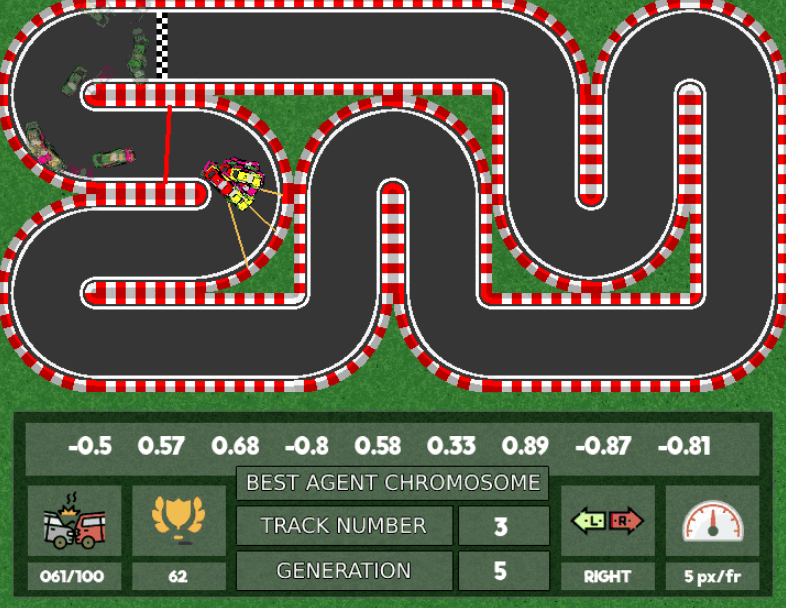
\includegraphics[width=70mm,scale=4]{assets/simulation.png}}
    \caption{Pygame simulation for the genetic algorithm}
    \label{fig:simulation}
\end{figure}

\subsection{Agent controller}
In a population of cars, there is an agent for each one of these cars. The Agent controls the car based on a value that
is applied to the car's rotation angle and this value corresponds to the output of the 2nd order polynomial function
math function \emph{w1*a + w2*b + w3*c + w5*a*c + w6*b*c + w7*a**2 + w8*b**2 + w9*c**2} where the inputs \emph{a, b, c} are
the distances of the car sensors at the moment and the weights will be the gene values of the Agent's current
chromosome. The returned value will be normalized to fit the range we are looking for (i.e. between -180 and 180) to be then applied
to the car's angle for the car to turn.


\subsection{Genetic algorithm}
For the genetic algorithm, it was established that the simulation would start with a population of 100 cars(A.1). Each car has an
agent that controls it. Each agent has a chromosome with 9 genes in it which corresponds to the 9 weights that will be applied to
car controller function (2nd polynomial) mentioned before.
Each gene has a value between -1 and 1 that is initially assigned randomly. After the current round ends: (A.2) all the agents are ranked
based on their fitness score which corresponds to the distance traveled by the car in the current round, and each car that crosses
the finish line its also compensated for it; (A.3) Between 15 and 40% of population agents are filtered out for a new generation;
(A.4) the top 2 parents crossover in a uniform way to give birth to new cars until we have 100 cars again; (A.5) a mutation
is made to every new child in a way that there's a fresh gene in every new child chromosome; (A.6) 10% of the cars are replaced with 
new fresh ones in order to avoid convergence.

\section{Experiments \& Results}
\subsection{Unwanted behaviour}
During the population evolution there were a few problems that were easily solved with a few tweaks on the code itself but after a few generations
some cars were behaving in a way that was not desired. The cars would tend to drive in circles or even drive in the opposite direction they were supposed to
be driving. This behaviour is a good example of what a good behavior for the agent can be not the desired one. This behavior would make the cars rank higher
in the population due to the distance traveled from the cars using this method. Of course, once a car finds this behavior, all the population tend to convergence
into that unwanted behaviour. To fix this problem, it was implemented a different type of car with a PID controller. Setting the controller setpoint
to the middle of the road and tweaking the components of the PID controller, made the car drive exactly as desired without crashing into the walls.
It was then attached to this PID controlled car a 'cleaner line' that would wipe out all the cars with unwanted behaviours (like those who were circling in a loop)
once the car collided with the line.

\begin{figure}[b]
    \centerline{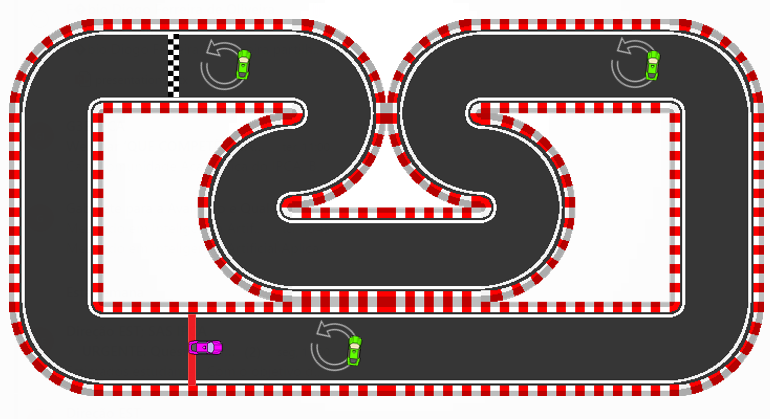
\includegraphics[width=70mm,scale=4]{assets/bad-behaviour.png}}
    \caption{Unwanted behaviour (cars spinning)}
    \label{fig:bad-behavious}
\end{figure}

\subsection{Results}
After this implementation all the simulation went well and after about 173 generations the car would now be able to drive perfectly without crashing and with
a better behaviour(faster) than the PID controlled car. The evolved agent was tested in every single track(beginner, easy, medium and hard) and managed to drive
perfectly in all of them.

\section{Conclusions}
Self-driving is still an active and emerging area in real-world applications. Although there's a lack of large-scale
public datasets available in order to train solid deep learning models. In this work, we showed how state-of-art methods can be
validated in the virtual world using serious games before being tested in the real world. Nowadays there's more advanced simulation
softwares that try to replicate the real world environment like CARLA software where its possible to test trained Deep Learning models
along with other usefull techniques. We hope, that this work motivates others to learn more about genetic algorithms and artificial
intelligence \cite{AIMA} in general.

\bibliographystyle{abbrv}
\bibliography{citations}

\vspace{12pt}
\end{document}
